\documentclass[10pt]{article}

\usepackage{multicol}
\usepackage[margin=0.75in]{geometry}
\usepackage{titlesec}
\usepackage{amsmath}
\usepackage[
backend=biber,
style=ieee,
sorting=ynt
]{biblatex}
\usepackage{fancyhdr}
\usepackage{enumitem}
\usepackage{graphicx}
\usepackage{float}

% \pagestyle{fancy}
%\fancyhf{}

\title{ECE419 M1 Report}
\date{28 January 2018}
\author{Thomas Kingsford\\Marcel Mongeon\\Zhihao Sheng}

%\titleformat{\section}{\normalfont\scshape}{\thesection}{1em}{}
%\titlespacing*{\section}{0pt}{10pt}{0pt}

%\setlength{\parindent}{0pt}
%\setlength{\parskip}{0cm}
%\renewcommand{\baselinestretch}{0.5}
%\setlist{noitemsep} % {nosep, noitemsep}

\begin{document}

\begin{multicols}{2}

\maketitle

\begin{figure}[H]
\centering
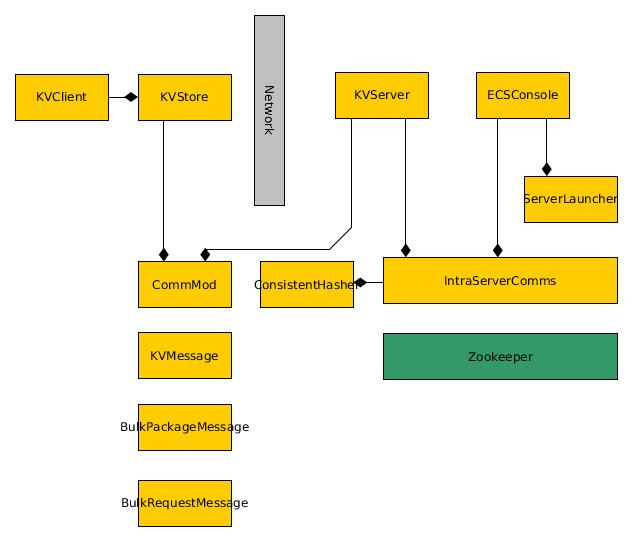
\includegraphics[scale=0.35]{m2_architecture}
\caption{Architecture Diagram}
\label{arch}
\end{figure}

\section{Design and Decisions}

\paragraph{Architecture and Preface} Refer to Figure \ref{arch} for an architecture diagram. This report focuses on the changes present in Milestone 2. Please refer to the Milestone 1 document for details about existing features and classes.

\paragraph{KVClient} The KVClient class handles client side interactions. It is left unchanged as additional milestone 2 logic is abstracted away inside KVStore and on the server side.

\paragraph{ConsistentHasher} The ConsistentHasher class implements logic to map keys to servers in the hash ring, as well as convenience functions to support the addition and removal of servers. Additionally, it supports serialization to allow the server ring to be sent in response to a request sent to the wrong server.

\paragraph{KVStore} The KVStore class handles the messages from the KVClient and passes them to the CommMod. It owns a ConsistentHasher object which is used to determine which server to send a request to. If ConsistentHasher is out of date, that server will respond with an updated ConsistentHasher, and the KVStore will issue an updated request. Notably, the KVStore exposes the same interface to the KVClient as in milestone 1. All key-to-server mapping occurs in KVStore without the knowledge of KVClient.

\paragraph{IntraServerComms} The IntraServerComms class provides an abstraction on top of ZooKeeper and provides the following functionality: Firstly, it provides subscribers with up-to-date ConsistentHasher instances. These instances are updated and distributed whenever ZooKeeper notifies IntraServerComms of a change in the server cluster (i.e. an added or removed server). Secondly, it provides a remote procedure call (RPC) interface from ECSConsole to named KVServers. This allows the ECSConsole to call the Start, Stop, LockWrite, UnlockWrite, and MoveData methods on the KVServer by using ZooKeeper.

\paragraph{KVServer} The KVServer class handles server side interface. It gets the KVMessage from KVClient through the CommMod and does the put or get request, then it will give the response to the KVClient through the CommMod.

\paragraph{CommMod} The CommMod class handles client and server communications. The server registers as a listener and receives KVMessages by way of a callback. The server must respond to each received KVMessage with a response message. Clients Connect() then send messages via SendMessage(), which returns a KVMessage response or else times out if the server fails to respond quickly enough. As of milestone 2, CommMod also supports the bulk sending and request of sets of tuples in single monolithic transactions, while enabling the sender and/or recipient to lock, as appropriate, to ensure data consistency. Such functionality is necessary to allow servers to be added or removed from the cluster.

\paragraph{BulkPackageMessage} Stores a set of tuples. Sent either in response to a BulkRequestMessage, or to hand off data without a corresponding request prior to a server being removed.

\paragraph{BulkRequestMessage} Represents a request for all tuples in an indicated hash range.

\paragraph{ServerLauncher} The ServerLauncher class exposes the functionality of launching and killing KVServer instances - on potentially remote servers - by way of SSH.

\paragraph{ECSConsole} The ECSConsole is an administrative user interface which enables a) automated testing by exposing a standard administrative API, and b) human administrative control of the server cluster - launching, starting and stopping servers and moving data.

\section{Test Cases}

\subsection{Milestone 1 Tests}

\paragraph{} The entire suite of unit tests from Milestone 1 remains, thus proving no regression of functionality.

\subsection{BulkMessageTest} Verifies the ability of BulkPackageMessages to (de)serialize their payload, among other things.

\subsection{ConsistentHasherTest} Verifies the ability of the ConsistentHasher to represent a set of servers, map keys to servers correctly, and other functionality.

\subsection{IntraServerCommsTest} Primarily validates the ability of IntraServerComms to provide remote procedure call (RPC) functionality, as well as to notify the listener of changes to the hash ring.

\subsection{StoreServerTests} Tests the complete KVStore-to-KVServer interaction including getting/putting/deleting tuples, requesting from an incorrect server, etc.

\subsection{ZooKeeperTest} Tests basic ZooKeeper functionality. Primarily used to verify that any failures in other tests aren't due to, for example, ZooKeeper not being started.

\section{Performance Evaluation}

%TODO

\end{multicols}

\end{document}

